% ============================================================
% LLM-BLM 実験 S4：過去の偏りで TE の上限を校正すると、小型株の BLM の実現の TE は約束の 3% に近づくか
% コンパイル：tectonic -X compile LLM-BLM_実験S4.tex   （XeTeX 系。このフォルダで実行する）
% 数値と表は 図/values.tex・図/tab_*.tex（作成スクリプト/values.py）、図は 図/*.pdf（作成スクリプト/figs.py）。
% どちらも experiments/S4_te_calibration/results から作る。本文に数値を手で書かない。
% ============================================================
\documentclass[xelatex,ja=standard,jafont=haranoaji,a4paper,10pt,openany]{bxjsreport}
\setpagelayout*{left=22mm,right=22mm,top=24mm,bottom=26mm,footskip=11mm}

\usepackage{amsmath,amssymb,mathtools,bm}
\usepackage{booktabs,array,multirow,longtable}
\usepackage{graphicx}
\usepackage{adjustbox}
\usepackage{xcolor}
\usepackage{enumitem}
\usepackage{caption}
\usepackage{float}
\usepackage[most]{tcolorbox}
\usepackage[hidelinks,bookmarksnumbered]{hyperref}

\graphicspath{{図/}}
% values.py が results から作る。手で直さない。
\expandafter\def\csname v@commit\endcsname{1e027b6}
\expandafter\def\csname v@primaryD\endcsname{$+$0.148}
\expandafter\def\csname v@primarylo\endcsname{$+$0.048}
\expandafter\def\csname v@primaryhi\endcsname{$+$0.180}
\expandafter\def\csname v@primaryp\endcsname{0.004}
\expandafter\def\csname v@primarygref\endcsname{1.22}
\expandafter\def\csname v@primarygnew\endcsname{1.05}
\expandafter\def\csname v@primarydays\endcsname{2,449}
\expandafter\def\csname v@primaryteref\endcsname{3.7\%}
\expandafter\def\csname v@primarytenew\endcsname{3.2\%}
\expandafter\def\csname v@AvsAcalD\endcsname{$+$0.186}
\expandafter\def\csname v@AvsAcallo\endcsname{$+$0.058}
\expandafter\def\csname v@AvsAcalhi\endcsname{$+$0.205}
\expandafter\def\csname v@AvsAcalp\endcsname{0.003}
\expandafter\def\csname v@AvsAcalgref\endcsname{1.26}
\expandafter\def\csname v@AvsAcalgnew\endcsname{1.04}
\expandafter\def\csname v@AvsAcaldays\endcsname{2,449}
\expandafter\def\csname v@AvsAcalteref\endcsname{3.8\%}
\expandafter\def\csname v@AvsAcaltenew\endcsname{3.1\%}
\expandafter\def\csname v@gptBvsBcalD\endcsname{$+$0.664}
\expandafter\def\csname v@gptBvsBcallo\endcsname{$+$0.042}
\expandafter\def\csname v@gptBvsBcalhi\endcsname{$+$0.926}
\expandafter\def\csname v@gptBvsBcalp\endcsname{0.017}
\expandafter\def\csname v@gptBvsBcalgref\endcsname{2.26}
\expandafter\def\csname v@gptBvsBcalgnew\endcsname{1.16}
\expandafter\def\csname v@gptBvsBcaldays\endcsname{565}
\expandafter\def\csname v@gptBvsBcalteref\endcsname{6.8\%}
\expandafter\def\csname v@gptBvsBcaltenew\endcsname{3.5\%}
\expandafter\def\csname v@AcalvsBcalD\endcsname{$-$0.009}
\expandafter\def\csname v@AcalvsBcallo\endcsname{$-$0.052}
\expandafter\def\csname v@AcalvsBcalhi\endcsname{$+$0.038}
\expandafter\def\csname v@AcalvsBcalp\endcsname{0.515}
\expandafter\def\csname v@AcalvsBcalgref\endcsname{1.04}
\expandafter\def\csname v@AcalvsBcalgnew\endcsname{1.05}
\expandafter\def\csname v@AcalvsBcaldays\endcsname{2,449}
\expandafter\def\csname v@AcalvsBcalteref\endcsname{3.1\%}
\expandafter\def\csname v@AcalvsBcaltenew\endcsname{3.2\%}
\expandafter\def\csname v@primaryverdict\endcsname{支持}
\expandafter\def\csname v@2015quarterchronoridgeAfinalvalue\endcsname{5.078}
\expandafter\def\csname v@2015quarterchronoridgeAterealizedeval\endcsname{3.8\%}
\expandafter\def\csname v@2015quarterchronoridgeAlimitmean\endcsname{3.0\%}
\expandafter\def\csname v@2015quarterchronoridgeAireval\endcsname{$+$0.93}
\expandafter\def\csname v@2015quarterchronoridgeAannualexcessoverband\endcsname{$+$2.8\%}
\expandafter\def\csname v@2015quarterchronoridgeAcalfinalvalue\endcsname{4.821}
\expandafter\def\csname v@2015quarterchronoridgeAcalterealizedeval\endcsname{3.1\%}
\expandafter\def\csname v@2015quarterchronoridgeAcallimitmean\endcsname{2.4\%}
\expandafter\def\csname v@2015quarterchronoridgeAcalireval\endcsname{$+$0.90}
\expandafter\def\csname v@2015quarterchronoridgeAcalannualexcessoverband\endcsname{$+$2.2\%}
\expandafter\def\csname v@2015quarterchronoridgeBfinalvalue\endcsname{5.171}
\expandafter\def\csname v@2015quarterchronoridgeBterealizedeval\endcsname{3.7\%}
\expandafter\def\csname v@2015quarterchronoridgeBlimitmean\endcsname{3.0\%}
\expandafter\def\csname v@2015quarterchronoridgeBireval\endcsname{$+$1.01}
\expandafter\def\csname v@2015quarterchronoridgeBannualexcessoverband\endcsname{$+$3.0\%}
\expandafter\def\csname v@2015quarterchronoridgeBcalfinalvalue\endcsname{4.899}
\expandafter\def\csname v@2015quarterchronoridgeBcalterealizedeval\endcsname{3.2\%}
\expandafter\def\csname v@2015quarterchronoridgeBcallimitmean\endcsname{2.5\%}
\expandafter\def\csname v@2015quarterchronoridgeBcalireval\endcsname{$+$0.96}
\expandafter\def\csname v@2015quarterchronoridgeBcalannualexcessoverband\endcsname{$+$2.4\%}
\expandafter\def\csname v@2015quarterband\endcsname{3.906}
\expandafter\def\csname v@2015halfchronoridgeAfinalvalue\endcsname{4.807}
\expandafter\def\csname v@2015halfchronoridgeAterealizedeval\endcsname{3.8\%}
\expandafter\def\csname v@2015halfchronoridgeAlimitmean\endcsname{3.0\%}
\expandafter\def\csname v@2015halfchronoridgeAireval\endcsname{$+$0.77}
\expandafter\def\csname v@2015halfchronoridgeAannualexcessoverband\endcsname{$+$2.4\%}
\expandafter\def\csname v@2015halfchronoridgeAcalfinalvalue\endcsname{4.581}
\expandafter\def\csname v@2015halfchronoridgeAcalterealizedeval\endcsname{3.1\%}
\expandafter\def\csname v@2015halfchronoridgeAcallimitmean\endcsname{2.4\%}
\expandafter\def\csname v@2015halfchronoridgeAcalireval\endcsname{$+$0.77}
\expandafter\def\csname v@2015halfchronoridgeAcalannualexcessoverband\endcsname{$+$1.9\%}
\expandafter\def\csname v@2015halfchronoridgeBfinalvalue\endcsname{4.788}
\expandafter\def\csname v@2015halfchronoridgeBterealizedeval\endcsname{3.8\%}
\expandafter\def\csname v@2015halfchronoridgeBlimitmean\endcsname{3.0\%}
\expandafter\def\csname v@2015halfchronoridgeBireval\endcsname{$+$0.80}
\expandafter\def\csname v@2015halfchronoridgeBannualexcessoverband\endcsname{$+$2.4\%}
\expandafter\def\csname v@2015halfchronoridgeBcalfinalvalue\endcsname{4.592}
\expandafter\def\csname v@2015halfchronoridgeBcalterealizedeval\endcsname{3.2\%}
\expandafter\def\csname v@2015halfchronoridgeBcallimitmean\endcsname{2.4\%}
\expandafter\def\csname v@2015halfchronoridgeBcalireval\endcsname{$+$0.79}
\expandafter\def\csname v@2015halfchronoridgeBcalannualexcessoverband\endcsname{$+$1.9\%}
\expandafter\def\csname v@2015halfband\endcsname{3.838}
\expandafter\def\csname v@2015yearchronoridgeAfinalvalue\endcsname{4.732}
\expandafter\def\csname v@2015yearchronoridgeAterealizedeval\endcsname{4.0\%}
\expandafter\def\csname v@2015yearchronoridgeAlimitmean\endcsname{3.0\%}
\expandafter\def\csname v@2015yearchronoridgeAireval\endcsname{$+$0.57}
\expandafter\def\csname v@2015yearchronoridgeAannualexcessoverband\endcsname{$+$1.6\%}
\expandafter\def\csname v@2015yearchronoridgeAcalfinalvalue\endcsname{4.603}
\expandafter\def\csname v@2015yearchronoridgeAcalterealizedeval\endcsname{3.2\%}
\expandafter\def\csname v@2015yearchronoridgeAcallimitmean\endcsname{2.3\%}
\expandafter\def\csname v@2015yearchronoridgeAcalireval\endcsname{$+$0.60}
\expandafter\def\csname v@2015yearchronoridgeAcalannualexcessoverband\endcsname{$+$1.3\%}
\expandafter\def\csname v@2015yearchronoridgeBfinalvalue\endcsname{4.782}
\expandafter\def\csname v@2015yearchronoridgeBterealizedeval\endcsname{3.9\%}
\expandafter\def\csname v@2015yearchronoridgeBlimitmean\endcsname{3.0\%}
\expandafter\def\csname v@2015yearchronoridgeBireval\endcsname{$+$0.62}
\expandafter\def\csname v@2015yearchronoridgeBannualexcessoverband\endcsname{$+$1.7\%}
\expandafter\def\csname v@2015yearchronoridgeBcalfinalvalue\endcsname{4.635}
\expandafter\def\csname v@2015yearchronoridgeBcalterealizedeval\endcsname{3.2\%}
\expandafter\def\csname v@2015yearchronoridgeBcallimitmean\endcsname{2.4\%}
\expandafter\def\csname v@2015yearchronoridgeBcalireval\endcsname{$+$0.64}
\expandafter\def\csname v@2015yearchronoridgeBcalannualexcessoverband\endcsname{$+$1.4\%}
\expandafter\def\csname v@2015yearband\endcsname{4.065}
\expandafter\def\csname v@2023quarterchronoridgeAfinalvalue\endcsname{1.873}
\expandafter\def\csname v@2023quarterchronoridgeAterealizedeval\endcsname{4.2\%}
\expandafter\def\csname v@2023quarterchronoridgeAlimitmean\endcsname{3.0\%}
\expandafter\def\csname v@2023quarterchronoridgeAireval\endcsname{$+$1.81}
\expandafter\def\csname v@2023quarterchronoridgeAannualexcessoverband\endcsname{$+$10.3\%}
\expandafter\def\csname v@2023quarterchronoridgeAcalfinalvalue\endcsname{1.804}
\expandafter\def\csname v@2023quarterchronoridgeAcalterealizedeval\endcsname{3.1\%}
\expandafter\def\csname v@2023quarterchronoridgeAcallimitmean\endcsname{2.2\%}
\expandafter\def\csname v@2023quarterchronoridgeAcalireval\endcsname{$+$1.87}
\expandafter\def\csname v@2023quarterchronoridgeAcalannualexcessoverband\endcsname{$+$8.6\%}
\expandafter\def\csname v@2023quarterchronoridgeBfinalvalue\endcsname{1.844}
\expandafter\def\csname v@2023quarterchronoridgeBterealizedeval\endcsname{3.8\%}
\expandafter\def\csname v@2023quarterchronoridgeBlimitmean\endcsname{3.0\%}
\expandafter\def\csname v@2023quarterchronoridgeBireval\endcsname{$+$1.84}
\expandafter\def\csname v@2023quarterchronoridgeBannualexcessoverband\endcsname{$+$9.6\%}
\expandafter\def\csname v@2023quarterchronoridgeBcalfinalvalue\endcsname{1.790}
\expandafter\def\csname v@2023quarterchronoridgeBcalterealizedeval\endcsname{3.3\%}
\expandafter\def\csname v@2023quarterchronoridgeBcallimitmean\endcsname{2.3\%}
\expandafter\def\csname v@2023quarterchronoridgeBcalireval\endcsname{$+$1.74}
\expandafter\def\csname v@2023quarterchronoridgeBcalannualexcessoverband\endcsname{$+$8.3\%}
\expandafter\def\csname v@2023quartergptridgeBfinalvalue\endcsname{1.538}
\expandafter\def\csname v@2023quartergptridgeBterealizedeval\endcsname{6.8\%}
\expandafter\def\csname v@2023quartergptridgeBlimitmean\endcsname{3.0\%}
\expandafter\def\csname v@2023quartergptridgeBireval\endcsname{$+$0.28}
\expandafter\def\csname v@2023quartergptridgeBannualexcessoverband\endcsname{$+$1.6\%}
\expandafter\def\csname v@2023quartergptridgeBcalfinalvalue\endcsname{1.550}
\expandafter\def\csname v@2023quartergptridgeBcalterealizedeval\endcsname{3.5\%}
\expandafter\def\csname v@2023quartergptridgeBcallimitmean\endcsname{2.3\%}
\expandafter\def\csname v@2023quartergptridgeBcalireval\endcsname{$+$0.62}
\expandafter\def\csname v@2023quartergptridgeBcalannualexcessoverband\endcsname{$+$2.0\%}
\expandafter\def\csname v@2023quarterband\endcsname{1.479}
\expandafter\def\csname v@2023halfchronoridgeAfinalvalue\endcsname{1.766}
\expandafter\def\csname v@2023halfchronoridgeAterealizedeval\endcsname{4.2\%}
\expandafter\def\csname v@2023halfchronoridgeAlimitmean\endcsname{3.0\%}
\expandafter\def\csname v@2023halfchronoridgeAireval\endcsname{$+$0.83}
\expandafter\def\csname v@2023halfchronoridgeAannualexcessoverband\endcsname{$+$6.9\%}
\expandafter\def\csname v@2023halfchronoridgeAcalfinalvalue\endcsname{1.780}
\expandafter\def\csname v@2023halfchronoridgeAcalterealizedeval\endcsname{3.5\%}
\expandafter\def\csname v@2023halfchronoridgeAcallimitmean\endcsname{2.3\%}
\expandafter\def\csname v@2023halfchronoridgeAcalireval\endcsname{$+$1.10}
\expandafter\def\csname v@2023halfchronoridgeAcalannualexcessoverband\endcsname{$+$7.2\%}
\expandafter\def\csname v@2023halfchronoridgeBfinalvalue\endcsname{1.766}
\expandafter\def\csname v@2023halfchronoridgeBterealizedeval\endcsname{4.0\%}
\expandafter\def\csname v@2023halfchronoridgeBlimitmean\endcsname{3.0\%}
\expandafter\def\csname v@2023halfchronoridgeBireval\endcsname{$+$0.94}
\expandafter\def\csname v@2023halfchronoridgeBannualexcessoverband\endcsname{$+$6.9\%}
\expandafter\def\csname v@2023halfchronoridgeBcalfinalvalue\endcsname{1.782}
\expandafter\def\csname v@2023halfchronoridgeBcalterealizedeval\endcsname{3.7\%}
\expandafter\def\csname v@2023halfchronoridgeBcallimitmean\endcsname{2.4\%}
\expandafter\def\csname v@2023halfchronoridgeBcalireval\endcsname{$+$1.14}
\expandafter\def\csname v@2023halfchronoridgeBcalannualexcessoverband\endcsname{$+$7.3\%}
\expandafter\def\csname v@2023halfgptridgeBfinalvalue\endcsname{1.451}
\expandafter\def\csname v@2023halfgptridgeBterealizedeval\endcsname{6.8\%}
\expandafter\def\csname v@2023halfgptridgeBlimitmean\endcsname{3.0\%}
\expandafter\def\csname v@2023halfgptridgeBireval\endcsname{$-$0.21}
\expandafter\def\csname v@2023halfgptridgeBannualexcessoverband\endcsname{$-$1.6\%}
\expandafter\def\csname v@2023halfgptridgeBcalfinalvalue\endcsname{1.484}
\expandafter\def\csname v@2023halfgptridgeBcalterealizedeval\endcsname{3.6\%}
\expandafter\def\csname v@2023halfgptridgeBcallimitmean\endcsname{2.4\%}
\expandafter\def\csname v@2023halfgptridgeBcalireval\endcsname{$-$0.11}
\expandafter\def\csname v@2023halfgptridgeBcalannualexcessoverband\endcsname{$-$0.7\%}
\expandafter\def\csname v@2023halfband\endcsname{1.508}
\expandafter\def\csname v@2023yearchronoridgeAfinalvalue\endcsname{1.683}
\expandafter\def\csname v@2023yearchronoridgeAterealizedeval\endcsname{4.6\%}
\expandafter\def\csname v@2023yearchronoridgeAlimitmean\endcsname{3.0\%}
\expandafter\def\csname v@2023yearchronoridgeAireval\endcsname{$+$0.04}
\expandafter\def\csname v@2023yearchronoridgeAannualexcessoverband\endcsname{$+$3.6\%}
\expandafter\def\csname v@2023yearchronoridgeAcalfinalvalue\endcsname{1.724}
\expandafter\def\csname v@2023yearchronoridgeAcalterealizedeval\endcsname{3.8\%}
\expandafter\def\csname v@2023yearchronoridgeAcallimitmean\endcsname{2.4\%}
\expandafter\def\csname v@2023yearchronoridgeAcalireval\endcsname{$+$0.30}
\expandafter\def\csname v@2023yearchronoridgeAcalannualexcessoverband\endcsname{$+$4.6\%}
\expandafter\def\csname v@2023yearchronoridgeBfinalvalue\endcsname{1.682}
\expandafter\def\csname v@2023yearchronoridgeBterealizedeval\endcsname{4.5\%}
\expandafter\def\csname v@2023yearchronoridgeBlimitmean\endcsname{3.0\%}
\expandafter\def\csname v@2023yearchronoridgeBireval\endcsname{$+$0.07}
\expandafter\def\csname v@2023yearchronoridgeBannualexcessoverband\endcsname{$+$3.6\%}
\expandafter\def\csname v@2023yearchronoridgeBcalfinalvalue\endcsname{1.718}
\expandafter\def\csname v@2023yearchronoridgeBcalterealizedeval\endcsname{3.6\%}
\expandafter\def\csname v@2023yearchronoridgeBcallimitmean\endcsname{2.5\%}
\expandafter\def\csname v@2023yearchronoridgeBcalireval\endcsname{$+$0.32}
\expandafter\def\csname v@2023yearchronoridgeBcalannualexcessoverband\endcsname{$+$4.5\%}
\expandafter\def\csname v@2023yeargptridgeBfinalvalue\endcsname{1.461}
\expandafter\def\csname v@2023yeargptridgeBterealizedeval\endcsname{3.7\%}
\expandafter\def\csname v@2023yeargptridgeBlimitmean\endcsname{3.0\%}
\expandafter\def\csname v@2023yeargptridgeBireval\endcsname{$-$0.61}
\expandafter\def\csname v@2023yeargptridgeBannualexcessoverband\endcsname{$-$2.5\%}
\expandafter\def\csname v@2023yeargptridgeBcalfinalvalue\endcsname{1.461}
\expandafter\def\csname v@2023yeargptridgeBcalterealizedeval\endcsname{3.3\%}
\expandafter\def\csname v@2023yeargptridgeBcallimitmean\endcsname{2.8\%}
\expandafter\def\csname v@2023yeargptridgeBcalireval\endcsname{$-$0.70}
\expandafter\def\csname v@2023yeargptridgeBcalannualexcessoverband\endcsname{$-$2.5\%}
\expandafter\def\csname v@2023yearband\endcsname{1.550}

\newcommand{\V}[1]{\ifcsname v@#1\endcsname\csname v@#1\endcsname\else\textbf{??#1??}\fi}
\newcommand{\tabin}[1]{\adjustbox{max width=\linewidth}{\input{図/tab_#1.tex}}}

\definecolor{c1}{HTML}{2A78D6}
\definecolor{soft1}{HTML}{E4EEF9}

\newcommand{\code}[1]{\texttt{#1}}
\newcommand{\SP}{S\&P500}
\newcommand{\figref}[1]{図~\ref{#1}}
\newcommand{\tabref}[1]{表~\ref{#1}}
\newcommand{\chapref}[1]{第~\ref{#1}~章}

\setlist[itemize]{leftmargin=1.6em,itemsep=0.2em,topsep=0.4em}
\setlist[enumerate]{leftmargin=1.8em,itemsep=0.2em,topsep=0.4em}
\captionsetup{font=small,labelfont=bf,skip=6pt}
\renewcommand{\arraystretch}{1.2}

\makeatletter
\def\@makechapterhead#1{\vspace*{0.3\Cvs}{\parindent\z@\raggedright\normalfont
  \ifnum\c@secnumdepth>\m@ne\if@mainmatter{\Large\headfont\@chapapp\thechapter\@chappos}\par\nobreak\vskip0.4\Cvs\fi\fi
  \interlinepenalty\@M\LARGE\headfont #1\par\nobreak\vskip 1.5\Cvs}}
\def\@makeschapterhead#1{\vspace*{0.3\Cvs}{\parindent\z@\raggedright\normalfont
  \interlinepenalty\@M\LARGE\headfont #1\par\nobreak\vskip 1.5\Cvs}}
\makeatother

\newtcolorbox{keybox}[1][要点]{enhanced,breakable,colback=soft1,colframe=c1,boxrule=0.5pt,arc=2pt,
  left=8pt,right=8pt,top=6pt,bottom=6pt,title={#1},fonttitle=\sffamily\bfseries\small,coltitle=white}

\title{LLM-BLM 実験 S4\\[6pt]
  \large 過去の偏りで TE の上限を校正すると、\\小型株の BLM の実現の TE は約束の 3\% に近づくか}
\author{実験の報告書（事前登録した検定の結果）}
\date{2026 年 10 月 25 日}

\begin{document}
\maketitle

\chapter*{概要}
\addcontentsline{toc}{chapter}{概要}

実験 S3 で、小型株の BLM の事前の TE は、実現の TE を小さく見積もっていた。この実験 S4 では、各リバランスの日に、その運用自身の過去 3 年の偏り（実現 ÷ 事前の TE の目安）で TE の上限を割る校正を入れ、実現の TE が約束の年 3\% に近づくかを、事前登録して 1 回だけ確かめた。

\begin{keybox}[要点]
\begin{itemize}
\item \textbf{主な検定は\V{primaryverdict}された}。株価で補正した共分散（S3 の B）に校正を足すと、2017 年以降の実現の TE は \V{primaryteref} から \V{primarytenew} になり、約束の 3\% にはっきり近づいた（片側 $p$ = \V{primaryp}）。
\item 補正なしの共分散でも（\V{AvsAcalteref} → \V{AvsAcaltenew}）、gpt-4o-mini の見通しでも（\V{gptBvsBcalteref} → \V{gptBvsBcaltenew}）、同じように効いた。
\item \textbf{校正した後は、共分散の補正の差はなくなった}（\V{AcalvsBcalteref} と \V{AcalvsBcaltenew}）。
\item \textbf{リスク 1 単位あたりの成績（情報レシオ）は保たれた}。リスクを小さくした分、比べる相手との差は小さくなった（2015 年末から四半期ごとで、年 \V{2015quarterchronoridgeBannualexcessoverband} → \V{2015quarterchronoridgeBcalannualexcessoverband}）。
\item \textbf{急な変化には追いつかない}。2020 年と 2025 年には、校正しても実現の TE が 4\% を超えた。
\item これからの BLM では、この校正を標準にする。
\end{itemize}
\end{keybox}


\setcounter{tocdepth}{1}
{\small\tableofcontents}

% ============================================================
\chapter{目的}\label{ch:purpose}

実験 S3 で、小型株の BLM の事前の TE は、実現の TE を小さく見積もっていた。偏り $b$（実現 ÷ 事前の TE の目安）は、どの組み合わせでも 1 を超えた。株価のデータで共分散を補正すると偏りは小さくなったが、1 には届かなかった。

\SP{} の補足実験 X03 では、過去 36 か月の「実現 ÷ 事前の TE」で上限を割るだけで、実現の TE が約束の 3\% にずっと近づいた。

\begin{keybox}[問い]
小型株の BLM で、その運用自身の過去の偏りで TE の上限を割ると、実現の TE は約束の年 3\% に近づくか。
\end{keybox}

% ============================================================
\chapter{事前登録と方法}\label{ch:method}

仮説・方法・判定の基準は \code{experiments/S4\_te\_calibration/preregistration.md} に書き、コード（\code{run.py}）と同じコミットで固定してから、1 回だけ実行した。実行に使ったコミットは \code{\V{commit}}。S1〜S3 と同じ 1,000 社で、S3 の結果（$b > 1$）を見た後に設計した。

\section{校正の規則}

各リバランスの日に、その運用自身の、それより前の日の標準化した超過リターン（超過リターン ÷ その日に有効だった事前の日次の TE）の直近 756 日（約 3 年）から、偏り $b_{\text{past}}$ を計算する。事前の TE の上限を $L = 3\% / b_{\text{past}}$ とし、$[1\%, 6\%]$ に丸める。過去の日が 126 日に満たないあいだは $L = 3\%$ のままにする。

\section{比べる組み合わせ}

ポートフォリオは S3 と同じ（範囲、リバランスの日、BLM、費用、比べる相手）。共分散は S3 の A（直近 252 日の Ledoit--Wolf）と B（株価のデータで補正）で、それぞれ校正なしと校正あり（\_cal）を作った。見通しは ChronoGPT＋リッジ（2015 年末と 2023 年末から）と、gpt-4o-mini（重みを学習、2023 年末から、B と B\_cal）。

\section{主な検定}

2015 年末から四半期ごと、ChronoGPT＋リッジの見通し、共分散 B で、校正なし（B）と校正あり（B\_cal）を比べる。2017 年以降の日について、約束に対する日次の比 $u_t$ = 超過リターン ÷ $(3\% / \sqrt{252})$ から $g = \sqrt{\overline{u_t^2}}$（$g = 1$ なら実現の TE がちょうど 3\%）を作り、$D = |\log g_B| - |\log g_{B\_cal}| > 0$ かを、S3 と同じブロック・ブートストラップで検定した（片側 $p < 0.05$ で「支持」）。

% ============================================================
% 結果の章（数値は 図/values.tex と 図/tab_*.tex から。手で書かない）

% ============================================================
\chapter{主な検定}\label{ch:primary}

\begin{table}[H]
\centering\small
\caption{実現の TE と約束（3\%）の近さ（$g$ = 実現の TE ÷ 3\% の目安。1 なら約束どおり）}
\label{tab:tests}
\begin{adjustbox}{max width=\linewidth}
\begin{tabular}{@{}lrrrrrr@{}}
\toprule
比べたもの & $g$（前） & $g$（後） & 実現の TE（前 → 後） & $D$ & 95\% 区間 & 片側 $p$ \\
\midrule
\textbf{主：B と B＋校正}（2015 年末から、\V{primarydays} 日） & \V{primarygref} & \V{primarygnew} & \V{primaryteref} → \V{primarytenew} & \V{primaryD} & [\V{primarylo}, \V{primaryhi}] & \V{primaryp} \\
副：A と A＋校正 & \V{AvsAcalgref} & \V{AvsAcalgnew} & \V{AvsAcalteref} → \V{AvsAcaltenew} & \V{AvsAcalD} & [\V{AvsAcallo}, \V{AvsAcalhi}] & \V{AvsAcalp} \\
副：gpt-4o-mini、B と B＋校正（2023 年末から、\V{gptBvsBcaldays} 日） & \V{gptBvsBcalgref} & \V{gptBvsBcalgnew} & \V{gptBvsBcalteref} → \V{gptBvsBcaltenew} & \V{gptBvsBcalD} & [\V{gptBvsBcallo}, \V{gptBvsBcalhi}] & \V{gptBvsBcalp} \\
副：A＋校正と B＋校正 & \V{AcalvsBcalgref} & \V{AcalvsBcalgnew} & \V{AcalvsBcalteref} → \V{AcalvsBcaltenew} & \V{AcalvsBcalD} & [\V{AcalvsBcallo}, \V{AcalvsBcalhi}] & \V{AcalvsBcalp} \\
\bottomrule
\end{tabular}
\end{adjustbox}
\end{table}

評価する日は、2015 年末からの版では 2017 年以降、2023 年末からの版では 2024 年 7 月以降。実現の TE は $3\% \times g$。

\begin{keybox}[結果]
主な検定は\textbf{\V{primaryverdict}}された。株価で補正した共分散（B）に校正を足すと、2017 年以降の実現の TE は \V{primaryteref} から \V{primarytenew} になり、約束の 3\% にはっきり近づいた（片側 $p$ = \V{primaryp}）。
\end{keybox}

\begin{itemize}
\item \textbf{補正なしの共分散（A）でも}、校正で実現の TE は \V{AvsAcalteref} から \V{AvsAcaltenew} に近づいた。
\item \textbf{gpt-4o-mini の見通し}では、実現の TE が \V{gptBvsBcalteref} から \V{gptBvsBcaltenew} へと、大きく改善した。
\item \textbf{校正した後は、共分散の補正の差はなくなった}（A＋校正 \V{AcalvsBcalteref}、B＋校正 \V{AcalvsBcaltenew}、片側 $p$ = \V{AcalvsBcalp}）。
\end{itemize}

% ============================================================
\chapter{上限と実現の TE の動き}\label{ch:te}

\begin{figure}[H]
\centering
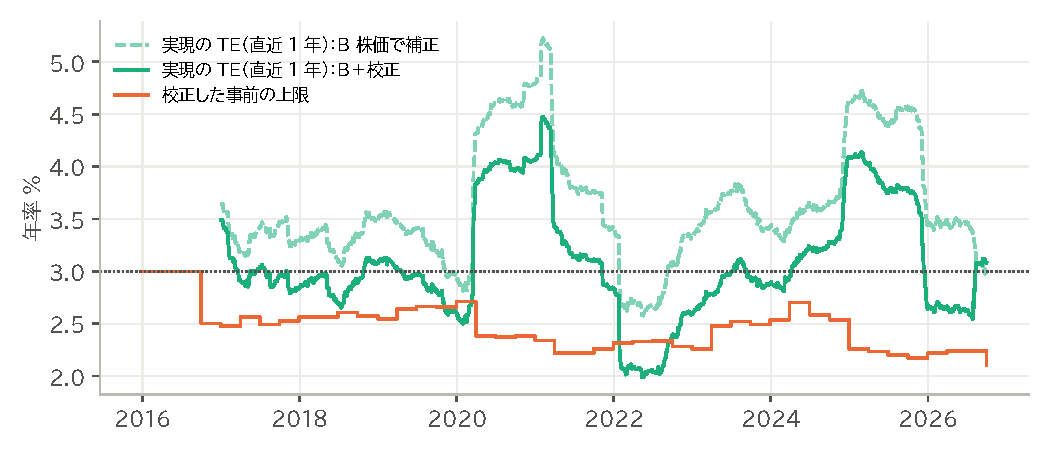
\includegraphics[width=\linewidth]{te.pdf}
\caption{2015 年末から四半期ごと、ChronoGPT＋リッジの見通し、共分散 B。直近 1 年の実現の TE（校正なしと校正あり）と、校正した事前の上限。点線は約束の 3\%。}
\label{fig:te}
\end{figure}

\begin{itemize}
\item 校正した上限は、多くの時期で年 2.1〜2.7\% だった（過去の偏りが 1.1〜1.4 程度で安定していた）。
\item それでも、2020 年の新型コロナの急落の後と、2025 年の前半には、実現の TE が 4\% を超えた。過去 3 年の偏りで割る規則は、変動が急に変わる時期には追いつかない（X03 と同じ）。
\item 落ち着いた時期（2018〜2019 年、2022〜2023 年）には、校正した版の実現の TE は 3\% の前後か、それより低かった。
\end{itemize}

% ============================================================
\chapter{すべての組み合わせ}\label{ch:runs}

\begin{table}[H]
\centering\small
\caption{2015 年 12 月末を 1 とした推移（2026 年 9 月末まで）。相手との差は年率。上限・実現の TE・$g$・情報レシオは評価する日（2017 年以降）のもの。情報レシオ = 比べる相手との差の年率 ÷ 実現の TE}
\label{tab:runs2015}
\tabin{runs_2015}
\end{table}

\begin{figure}[H]
\centering
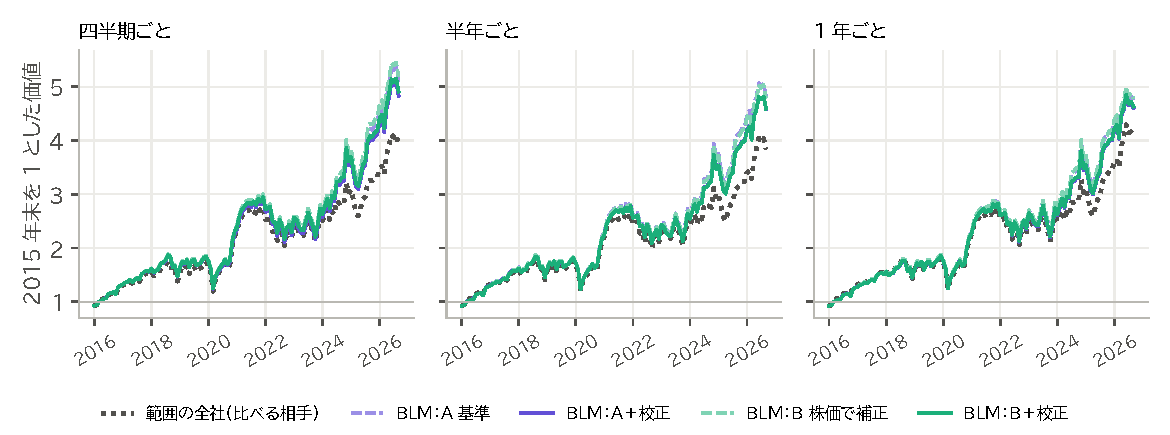
\includegraphics[width=\linewidth]{paths_2015_chrono_ridge.pdf}
\caption{2015 年末を 1 とした推移（ChronoGPT＋リッジの見通し）。}
\label{fig:paths2015}
\end{figure}

\begin{table}[H]
\centering\small
\caption{2023 年 12 月末を 1 とした推移（2026 年 9 月末まで）。上限・実現の TE・$g$・情報レシオは 2024 年 7 月以降}
\label{tab:runs2023}
\tabin{runs_2023}
\end{table}

\begin{figure}[H]
\centering
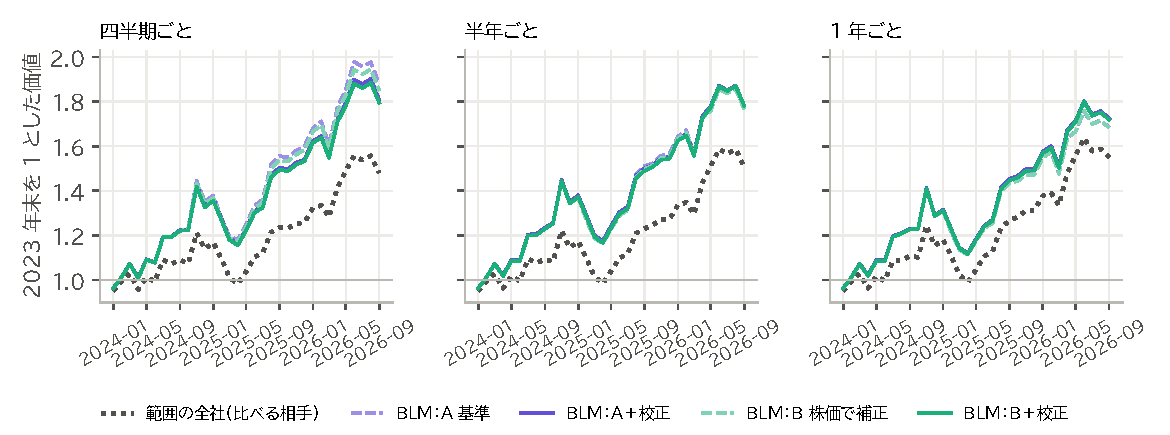
\includegraphics[width=\linewidth]{paths_2023_chrono_ridge.pdf}
\caption{2023 年末を 1 とした推移（ChronoGPT＋リッジの見通し）。}
\label{fig:paths2023c}
\end{figure}

\begin{figure}[H]
\centering
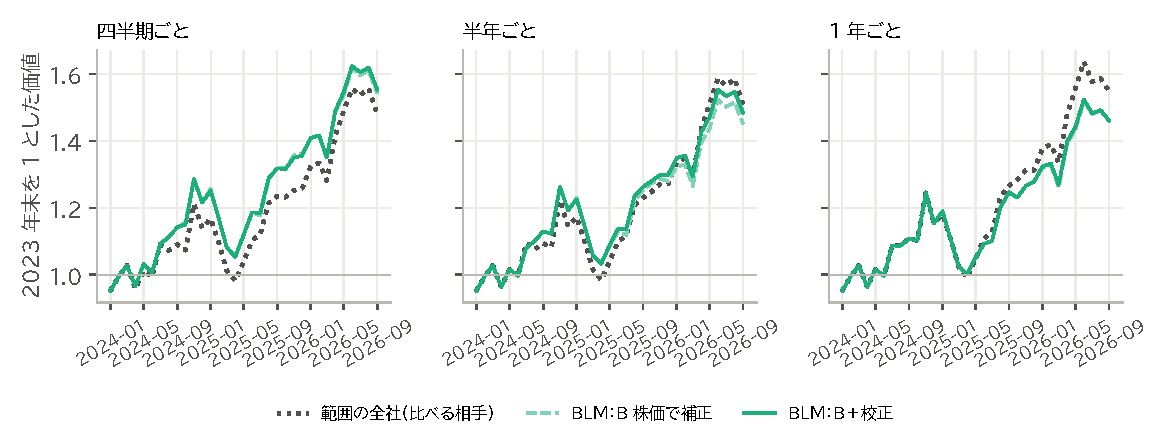
\includegraphics[width=\linewidth]{paths_2023_gpt_ridge.pdf}
\caption{2023 年末を 1 とした推移（gpt-4o-mini（重みを学習）の見通し）。}
\label{fig:paths2023g}
\end{figure}

\section{リスクとリターンの交換}

\begin{itemize}
\item 校正はリスクを小さくするので、比べる相手との差も小さくなる。2015 年末から四半期ごと（共分散 B）では、最終の値が \V{2015quarterchronoridgeBfinalvalue} から \V{2015quarterchronoridgeBcalfinalvalue}、相手との差が年 \V{2015quarterchronoridgeBannualexcessoverband} から \V{2015quarterchronoridgeBcalannualexcessoverband} になった。
\item リスク 1 単位あたり（情報レシオ）は、ほぼ変わらなかった（\V{2015quarterchronoridgeBireval} から \V{2015quarterchronoridgeBcalireval}。半年・1 年ごとでもほぼ同じか、わずかに良い）。
\item gpt-4o-mini の見通しでは、校正で情報レシオが良くなった（四半期ごとで \V{2023quartergptridgeBireval} から \V{2023quartergptridgeBcalireval}）。校正なしでは、事前の見積もりの 2 倍を超えるリスクを取っていた。
\end{itemize}

% ============================================================
\chapter{解釈}\label{ch:interpret}

\begin{enumerate}
\item \textbf{校正は効く}。過去 3 年の偏りで上限を割るだけで、実現の TE は約束の 3\% に近づいた。S\&P500 の X03 と同じ結果が、小型株の BLM でも、見通し（ChronoGPT・gpt-4o-mini）や共分散の作り方によらず得られた。
\item \textbf{校正した後は、共分散の補正（S3 の B）の差はなくなった}。S3 で B が偏りを小さくしたのは確かだが、その分は校正が吸収する。共分散の補正は、校正の前の「偏りの大きさ」を小さくするが、校正の後の「約束の守り方」は変えない。
\item \textbf{情報レシオは保たれた}。校正は、リスクとリターンを同じ割合で縮めるので、リスク 1 単位あたりの成績はほぼ変わらない。事前の見積もりが大きく外れていた gpt-4o-mini の見通しでは、むしろ良くなった。
\item \textbf{急な変化には追いつかない}。2020 年と 2025 年には、校正しても実現の TE が 4\% を超えた。過去の偏りを使う規則の限界である。
\end{enumerate}

\section{これからの BLM の標準}

\begin{itemize}
\item TE の上限に、この校正（過去 756 日の偏りで割る）を入れる。将来のデータを使わない規則なので、そのまま使える。
\item 報告書では「事前の TE の上限 3\%」でなく、「実現の TE はおよそ 3\%（評価する期間で \V{primarytenew}）」と書けるようになる。
\item 急な変化への対応（例えば VIX や直近 1 か月の変動率で上限を一時的に下げる、X04 の考え方）は、次の候補である。
\end{itemize}


% ============================================================
\chapter{限界}\label{ch:limits}

\begin{itemize}
\item \textbf{同じ 1,000 社}：S1〜S3 と同じ標本で、今も上場している会社だけである。
\item \textbf{規則は 1 つ}：756 日・126 日・$[1\%, 6\%]$ の組み合わせだけを試した。選び直すと過剰適合になる。
\item \textbf{リスクとリターンの交換}：校正はリスクを小さくした分だけ、比べる相手との差も小さくする。
\item \textbf{2023 年末からの版}は、校正が働く期間が短い。
\end{itemize}

% ============================================================
\chapter*{再現の手順}
\addcontentsline{toc}{chapter}{再現の手順}

リポジトリの直下で（\code{.venv} の Python）、S1・S2 の \code{run.py} の後に：

\begin{enumerate}
\item \code{python experiments/S4\_te\_calibration/run.py}（結果は \code{results/}。2 回目は summary.json があると止まる）。
\item \code{資料集/02\_実験/実験S4\_TEの校正/作成スクリプト/} の \code{values.py} と \code{figs.py}。
\item このフォルダで \code{tectonic -X compile LLM-BLM\_実験S4.tex}。
\end{enumerate}

\end{document}
